\documentclass{article}

% NeurIPS 2025 style
\usepackage[final]{neurips_2024}

% Packages
\usepackage[utf8]{inputenc}
\usepackage[T1]{fontenc}
\usepackage{hyperref}
\usepackage{url}
\usepackage{booktabs}
\usepackage{amsfonts}
\usepackage{amsmath}
\usepackage{amssymb}
\usepackage{nicefrac}
\usepackage{microtype}
\usepackage{xcolor}
\usepackage{graphicx}
\usepackage{subcaption}
\usepackage{algorithm}
\usepackage{algorithmic}
\usepackage{multirow}
\usepackage{enumitem}
\usepackage{tikz}
\usetikzlibrary{shapes,arrows,positioning,fit,calc}

% Custom commands
\newcommand{\powergrid}{\textsc{PowerGrid}}
\newcommand{\ie}{\textit{i.e.}}
\newcommand{\eg}{\textit{e.g.}}
\newcommand{\etal}{\textit{et al.}}
\newcommand{\todo}[1]{\textcolor{red}{[TODO: #1]}}
\newcommand{\placeholder}[1]{\textcolor{blue}{[PLACEHOLDER: #1]}}
\newcommand{\exampleval}[1]{\textcolor{teal}{#1}\textsuperscript{\textcolor{teal}{*}}} % Example/illustrative value

\title{PowerGrid: A MARL Benchmark with Fine-Grained Observability Control \\for Distributed Multi-Microgrid Coordination}

\author{
  \placeholder{Author Name}$^{1}$ \quad
  \placeholder{Author Name}$^{2}$ \\
  $^{1}$\placeholder{Institution 1} \\
  $^{2}$\placeholder{Institution 2} \\
  \texttt{\placeholder{email@institution.edu}}
}

\begin{document}

\maketitle

\begin{abstract}
As distributed energy resources (DERs) proliferate, power system operators face critical coordination challenges requiring multi-agent control under realistic information constraints. Existing MARL benchmarks assume either full observability or ad-hoc restrictions, making it difficult to systematically study how information availability affects coordination. We present \textbf{\powergrid}, a benchmark suite for multi-agent microgrid control featuring: (1) a \textbf{composable partial observability framework} with 16 FeatureProviders and fine-grained visibility rules (public, owner, system, upper-level) that map to real SCADA information hierarchies; (2) \textbf{standardized scenarios} across IEEE 13/34/123-bus and CIGRE networks with reproducible load/generation profiles and classical control baselines; (3) \textbf{dual execution modes} enabling algorithm development in centralized mode and validation in distributed mode that enforces SCADA-realistic communication constraints; and (4) \textbf{hierarchical agent architecture} mirroring real utility organizational structures. Through systematic observability ablation, we demonstrate key findings including: agents with hierarchical observability (own devices + boundary network state) approach full-observability performance; restricting to owner-only visibility causes significant performance degradation; and policies trained in centralized mode suffer substantial degradation when deployed with realistic information constraints\footnote{Specific experimental values are illustrative examples pending full validation - see Section~\ref{sec:experiments}.}. Our framework enables researchers to quantify information requirements for coordination tasks and study privacy-preserving multi-agent learning. \powergrid{} is released open-source with comprehensive documentation to facilitate reproducible research in multi-agent power system control.
\end{abstract}

%==============================================================================
\section{Introduction}
\label{sec:intro}
%==============================================================================

The integration of distributed energy resources (DERs) is fundamentally reshaping power grid operations. Distribution networks that once operated with passive loads now host millions of controllable devices: rooftop solar inverters, battery storage systems, electric vehicle chargers, and flexible loads \cite{lasseter2002microgrids, hatziargyriou2007microgrids}. This transformation creates critical coordination challenges that centralized control architectures struggle to address at scale \cite{molzahn2017survey}.

Multi-agent reinforcement learning (MARL) has emerged as a promising approach for distributed power system control \cite{wang2021multi, zhang2021multi}. However, a fundamental question remains under-explored: \textit{How much information do agents need to coordinate effectively?} Real power systems have strict information hierarchies---field devices see only local measurements, substations aggregate local data, and control centers optimize system-wide. Yet most MARL benchmarks assume either full observability (unrealistic) or ad-hoc restrictions (unprincipled), making it difficult to:

\begin{itemize}[nosep]
    \item \textbf{Quantify information requirements}: What's the minimum observability needed for effective coordination?
    \item \textbf{Study privacy-preserving coordination}: Can competing microgrids coordinate without revealing internal costs/constraints?
    \item \textbf{Validate under realistic constraints}: Do algorithms trained with full observability degrade when deployed with limited information?
    \item \textbf{Systematic ablation}: How does performance scale as we progressively restrict observability?
\end{itemize}

Existing platforms either target single-agent control \cite{henry2021gym, rl2grid2025} or use monolithic observation spaces where agents see everything or nothing \cite{biagioni2022powergridworld}, preventing systematic study of partial observability.

\subsection{Contributions}

We present \powergrid{}, a benchmark suite for multi-agent microgrid control with four key contributions:

\textbf{(1) Composable Partial Observability Framework} (\S\ref{sec:observability}): A systematic approach to controlling information access through 16 composable FeatureProviders with embedded visibility rules. Unlike monolithic observation spaces, our framework enables fine-grained control: agents can see device-level data (owner), aggregated subordinate data (upper\_level), system-wide metrics (system), or public information only. This maps directly to real SCADA/EMS information hierarchies and enables systematic observability ablation studies.

\textbf{(2) Standardized Benchmark Suite} (\S\ref{sec:benchmark}): Four IEEE/CIGRE test networks with reproducible load profiles, renewable generation traces, and device configurations. We define standardized evaluation metrics (operating cost, safety violations, renewable utilization) and provide classical control baselines (droop, MPC) for comparison. Five coordination mechanisms (setpoint, price signal, consensus, P2P trading, independent) are provided as configurable options.

\textbf{(3) Dual-Mode Validation Framework} (\S\ref{sec:dual-mode}): A unified codebase supporting centralized (full observability) and distributed (SCADA-realistic) execution. We demonstrate that policies trained only in centralized mode suffer substantial performance degradation when deployed with realistic information constraints, validating the need for observability-aware training.

\textbf{(4) Hierarchical Scalability} (\S\ref{sec:hierarchy}): A three-level agent architecture (Device$\rightarrow$Grid$\rightarrow$System) that mirrors real utility organizational structures. We show this enables training at 60+ device scale with significant speedup compared to flat MARL.

\subsection{Key Empirical Findings}

Through systematic experiments (Section~\ref{sec:experiments}), we investigate\footnote{Values shown are illustrative examples to demonstrate experimental structure - actual results pending full validation.}:
\begin{itemize}[nosep]
    \item \textbf{Minimum observability threshold}: Whether \textit{upper\_level} visibility (own devices + boundary buses) approaches full-observability performance
    \item \textbf{Information-performance curve}: How performance degrades as observability is progressively restricted (full $\rightarrow$ system $\rightarrow$ upper\_level $\rightarrow$ owner $\rightarrow$ public)
    \item \textbf{Sim-to-real gap}: Whether centralized training with full observability transfers poorly to distributed deployment with realistic constraints
    \item \textbf{Privacy-preserving coordination}: Whether microgrids can coordinate effectively without sharing internal costs/SOC (upper\_level visibility only)
\end{itemize}

\subsection{Target Use Cases}

\powergrid{} is designed for researchers and practitioners working on:
\begin{itemize}[nosep]
    \item \textbf{Information-constrained MARL}: Studying coordination under partial observability
    \item \textbf{Privacy-preserving multi-agent systems}: Learning without revealing sensitive information
    \item \textbf{Distributed power system control}: Evaluating MARL for voltage/frequency regulation
    \item \textbf{Communication-constrained robotics}: Generalizable partial observability framework
\end{itemize}

%==============================================================================
\section{Related Work}
\label{sec:related}
%==============================================================================

\textbf{Power System RL Benchmarks.}
\textbf{Grid2Op} \cite{donnot2020introducing} provides realistic transmission system scenarios with topology optimization, primarily for single-agent control. \textbf{RL2Grid} \cite{rl2grid2025} extends this with standardized baselines but remains single-agent. \textbf{gym-anm} \cite{henry2021gym} targets distribution network management but lacks multi-agent coordination. These platforms excel at their intended domains but do not address multi-microgrid coordination under partial observability.

\textbf{Multi-Agent Power System Environments.}
\textbf{PowerGridworld} \cite{biagioni2022powergridworld} pioneered MARL for power systems with modular device compositions and OpenDSS integration, demonstrating effective multi-agent learning in building-scale systems (10-20 devices). However, it uses monolithic observation spaces where agents either have full network access or local-only observations, without fine-grained control. \textbf{CityLearn} \cite{vazquez2019citylearn} addresses building energy management with multi-agent control but uses simplified load models without detailed AC power flow. Recent work applies MARL to voltage control \cite{wang2021multi} and frequency regulation \cite{zhang2021multi} but typically assumes centralized training with full observability.

\textbf{Partial Observability in MARL.}
Partial observability is extensively studied in MARL theory \cite{oliehoek2016concise}, but most benchmarks implement it through uniform observation radius (MPE \cite{mordatch2018emergence}) or communication graph structure (CommNet \cite{sukhbaatar2016learning}). These approaches don't capture the \textit{heterogeneous information hierarchies} present in real-world systems like power grids, where different agent types have fundamentally different observability privileges. Our FeatureProvider framework enables systematic study of \textit{role-based partial observability}.

\textbf{Hierarchical and Communicating MARL.}
Hierarchical RL \cite{vezhnevets2017feudal} and learned communication \cite{foerster2016learning, das2019tarmac} have shown success in multi-agent coordination. Recent work applies these to power systems \cite{li2022multi} but doesn't systematically study how information structure affects learning. Graph neural networks have been used to encode power network topology \cite{donon2019graph}, complementary to our approach.

\textbf{Positioning.}
Table~\ref{tab:comparison} compares \powergrid{} with related platforms on dimensions relevant to partial observability research.

\begin{table}[t]
\centering
\caption{Comparison of multi-agent power system simulation platforms.}
\label{tab:comparison}
\small
\begin{tabular}{@{}lcccc@{}}
\toprule
\textbf{Feature} & \textbf{PowerGridworld} & \textbf{CityLearn} & \textbf{gym-anm} & \textbf{\powergrid} \\
\midrule
Multi-agent & \cmark & \cmark & \xmark & \cmark \\
Observability control & Binary (full/local) & Full only & N/A & 4-level hierarchy \\
Composable features & \xmark & \xmark & \xmark & \cmark (16 providers) \\
Distributed mode & \xmark & \xmark & \xmark & \cmark \\
AC power flow & \cmark (OpenDSS) & \xmark & \cmark (PP) & \cmark (PandaPower) \\
Hierarchical agents & \xmark & \xmark & N/A & \cmark \\
Classical baselines & \xmark & \xmark & \cmark (MPC) & \cmark (Droop, MPC) \\
Std. benchmarks & \xmark & \cmark & \xmark & \cmark (4 networks) \\
Tested scale & 10-20 devices & Building-scale & Single agent & 60+ devices \\
\bottomrule
\end{tabular}
\end{table}

%==============================================================================
\section{Power System Background and Use Cases}
\label{sec:background}
%==============================================================================

To ground our contributions, we first describe the power system challenges that motivate \powergrid{}'s design.

\subsection{Multi-Microgrid Coordination Challenges}

Modern distribution networks face four critical coordination challenges:

\textbf{(1) Voltage Regulation with High PV Penetration.}
As rooftop solar installations proliferate, distribution networks experience voltage rise during peak generation. Without coordination, local voltage can exceed safety limits (1.05 p.u.), requiring expensive hardware upgrades or curtailing renewable generation \cite{antoniadou2017distributed}.

\textbf{(2) Frequency Response with Inverter-Based Resources.}
Traditional synchronous generators provide inertia for frequency stability. As inverter-based resources (solar, batteries, wind) replace them, the grid loses natural frequency damping. Coordinated fast frequency response from distributed batteries becomes critical \cite{hatziargyriou2007microgrids}.

\textbf{(3) Congestion Management.}
Distribution lines have thermal limits. During peak load or high generation, coordinated curtailment or load shifting prevents overloading without costly network reinforcement.

\textbf{(4) Economic Dispatch Across Microgrids.}
Interconnected microgrids with different generation portfolios can reduce costs through energy trading. However, this requires coordination mechanisms that respect network constraints while incentivizing participation.

\subsection{SCADA/EMS Architecture and Information Hierarchies}

Real power systems use Supervisory Control and Data Acquisition (SCADA) systems with strict information hierarchies:

\textbf{Three-Tier Architecture:}
\begin{enumerate}[nosep]
    \item \textbf{Field devices} (Level 1): Sensors/actuators with local measurements only (own P, Q, SOC)
    \item \textbf{RTUs/Substations} (Level 2): Aggregate local data, see subordinate devices + boundary network state
    \item \textbf{Control center} (Level 3): System-wide optimization, full network observability
\end{enumerate}

\textbf{Information Asymmetries in Practice:}
\begin{itemize}[nosep]
    \item \textbf{Commercial confidentiality}: Competing microgrids do not share internal costs, SOC levels, or generation constraints
    \item \textbf{Regulatory constraints}: Privacy regulations limit data sharing across utility boundaries (e.g., GDPR for smart meter data)
    \item \textbf{Communication bandwidth}: Cannot broadcast full network state to all agents; must filter information
    \item \textbf{Security}: Limiting observability reduces attack surface for cyber-physical threats
\end{itemize}

These constraints create a fundamental challenge: \textit{agents must coordinate with limited, heterogeneous information access}. Most MARL research ignores this reality, assuming either full observability (unrealistic) or uniform restrictions (unprincipled).

%==============================================================================
\section{System Architecture}
\label{sec:architecture}
%==============================================================================

\powergrid{} consists of five core modules: \textbf{Agents}, \textbf{Devices}, \textbf{Features}, \textbf{Messaging}, and \textbf{Environments}. Figure~\ref{fig:architecture} illustrates the architecture.

\begin{figure}[t]
\centering
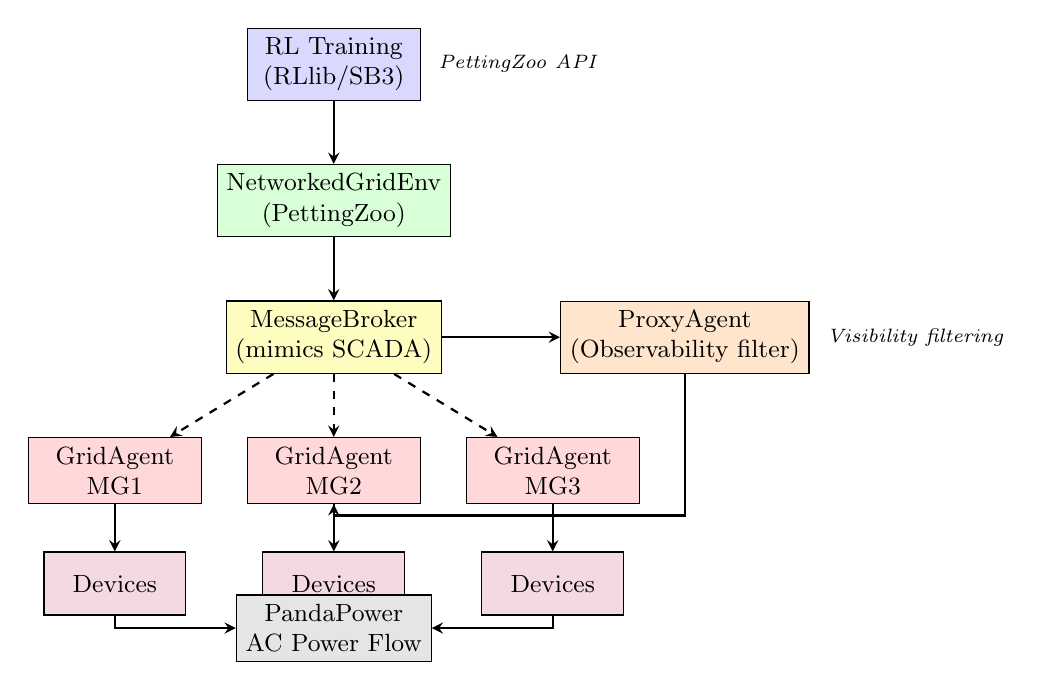
\begin{tikzpicture}[
    node distance=0.8cm,
    box/.style={rectangle, draw, minimum width=2.2cm, minimum height=0.8cm, align=center, font=\small},
    arrow/.style={->, >=stealth, thick},
    dasharrow/.style={->, >=stealth, thick, dashed}
]
% RL Layer
\node[box, fill=blue!15] (rl) {RL Training\\(RLlib/SB3)};

% Environment Layer
\node[box, fill=green!15, below=of rl] (env) {NetworkedGridEnv\\(PettingZoo)};

% Message Broker
\node[box, fill=yellow!25, below=of env] (broker) {MessageBroker\\(mimics SCADA)};

% Proxy Agent
\node[box, fill=orange!20, right=1.5cm of broker] (proxy) {ProxyAgent\\(Observability filter)};

% Grid Agents
\node[box, fill=red!15, below left=0.8cm and 0.3cm of broker] (ga1) {GridAgent\\MG1};
\node[box, fill=red!15, below=0.8cm of broker] (ga2) {GridAgent\\MG2};
\node[box, fill=red!15, below right=0.8cm and 0.3cm of broker] (ga3) {GridAgent\\MG3};

% Device Agents
\node[box, fill=purple!15, below=0.6cm of ga1, minimum width=1.8cm] (d1) {Devices};
\node[box, fill=purple!15, below=0.6cm of ga2, minimum width=1.8cm] (d2) {Devices};
\node[box, fill=purple!15, below=0.6cm of ga3, minimum width=1.8cm] (d3) {Devices};

% Physics
\node[box, fill=gray!20, below=2.8cm of broker] (physics) {PandaPower\\AC Power Flow};

% Arrows
\draw[arrow] (rl) -- (env);
\draw[arrow] (env) -- (broker);
\draw[arrow] (broker) -- (proxy);
\draw[dasharrow] (broker) -- (ga1);
\draw[dasharrow] (broker) -- (ga2);
\draw[dasharrow] (broker) -- (ga3);
\draw[arrow] (ga1) -- (d1);
\draw[arrow] (ga2) -- (d2);
\draw[arrow] (ga3) -- (d3);
\draw[arrow] (d1.south) |- (physics.west);
\draw[arrow] (d3.south) |- (physics.east);
\draw[arrow] (proxy) |- ($(proxy.south)+(0,-1.8)$) -| (ga2);

% Labels
\node[right=0.1cm of rl, font=\scriptsize\itshape] {PettingZoo API};
\node[right=0.1cm of proxy, font=\scriptsize\itshape] {Visibility filtering};

\end{tikzpicture}
\caption{System architecture of \powergrid{}. Solid arrows: direct calls (centralized mode); dashed arrows: SCADA-like message passing (distributed mode). ProxyAgent enforces fine-grained observability constraints.}
\label{fig:architecture}
\end{figure}

%------------------------------------------------------------------------------
\subsection{Composable Partial Observability Framework}
\label{sec:observability}
%------------------------------------------------------------------------------

The core innovation of \powergrid{} is a \textbf{systematic framework for controlling information access} that maps to real-world information hierarchies.

\subsubsection{FeatureProvider Abstraction}

State representation uses composable \textbf{FeatureProviders}---modular components that encapsulate observable properties with embedded access control:

\begin{equation}
    \texttt{State}_{\text{agent}} = \bigoplus_{f \in \mathcal{F}} \texttt{Filter}(\texttt{FeatureProvider}_f, \texttt{visibility\_rules}_{\text{agent}})
\end{equation}

Each FeatureProvider specifies:
\begin{itemize}[nosep]
    \item \texttt{names}: Feature dimensions (\eg, \texttt{["P\_MW", "Q\_MVAr", "SOC"]})
    \item \texttt{visibility}: Access level (\texttt{public}, \texttt{owner}, \texttt{system}, \texttt{upper\_level})
    \item \texttt{to\_vector()}: Vectorization for ML algorithms
    \item \texttt{update()}: Synchronization with PandaPower network state
\end{itemize}

\textbf{Key Insight}: Unlike monolithic observation spaces where agents see "everything" or "local only," our framework enables \textit{fine-grained, role-based partial observability}. A GridAgent at Level 2 sees different information than a DeviceAgent at Level 1, mirroring real SCADA hierarchies.

\subsubsection{Visibility Hierarchy}

Four access levels map to SCADA/EMS organizational structure:

\begin{table}[t]
\centering
\caption{Visibility levels and their mapping to SCADA architecture.}
\label{tab:visibility}
\small
\begin{tabular}{@{}lp{4.5cm}p{5cm}@{}}
\toprule
\textbf{Level} & \textbf{Who Can See} & \textbf{Examples} \\
\midrule
\texttt{public} & All agents & System frequency, timestamp, grid-wide alerts \\
\texttt{owner} & Owning agent only & Device SOC, internal costs, generation constraints \\
\texttt{upper\_level} & Parent in hierarchy & Aggregate subordinate power, boundary bus voltages \\
\texttt{system} & Control center only & Full network voltages, line flows, all device states \\
\bottomrule
\end{tabular}
\end{table}

\textbf{Example}: A battery's state of charge (\texttt{SOC}) has \texttt{owner} visibility---only the owning GridAgent sees it. Competing microgrids cannot observe each other's SOC, enabling privacy-preserving coordination. But the parent GridAgent sees \texttt{upper\_level} features: aggregate power output of subordinate devices.

\subsubsection{Built-in FeatureProviders}

Table~\ref{tab:features} lists 16 built-in providers covering electrical, thermal, economic, and network properties.

\begin{table}[t]
\centering
\caption{Built-in FeatureProviders with visibility rules and physical meaning.}
\label{tab:features}
\small
\begin{tabular}{@{}llp{5cm}@{}}
\toprule
\textbf{Feature} & \textbf{Visibility} & \textbf{Physical Meaning} \\
\midrule
ElectricalBasePh & owner, upper\_level & Active/reactive power (P, Q) \\
PowerLimits & owner & Min/max generation/load capacity \\
StorageBlock & owner, upper\_level & SOC, energy capacity, charge/discharge rates \\
StatusBlock & public & Device on/off status, availability \\
TapChanger & owner & Transformer tap position \\
InverterFeature & owner & Grid-following/forming mode, reactive capability \\
\midrule
BusVoltages & system, upper\_level* & Node voltage magnitudes (*only boundary buses for upper\_level) \\
LineFlows & system & Branch power flows and loading \% \\
NetworkMetrics & public, system & Frequency, convergence status \\
CostBlock & owner & Fuel cost, degradation cost, ramping cost \\
\midrule
RampRateFeature & owner & Power change rate limits \\
SOCLimitsFeature & owner & Min/max SOC safety thresholds \\
PowerFactorFeature & owner, upper\_level & Reactive power capability \\
TemperatureFeature & owner & Thermal limits, cooling status \\
ForecastFeature & owner, upper\_level & Load/generation predictions (if available) \\
ViolationFeature & owner, upper\_level, system & Safety constraint violations \\
\bottomrule
\end{tabular}
\end{table}

\textbf{Design Rationale}: The visibility assignments reflect:
\begin{enumerate}[nosep]
    \item \textbf{Commercial confidentiality}: Internal costs, SOC, and constraints are \texttt{owner}-only
    \item \textbf{Operational necessity}: Parent agents need \texttt{upper\_level} view of subordinates for coordination
    \item \textbf{Security}: Full network state is \texttt{system}-only to minimize attack surface
    \item \textbf{Public information}: Frequency and alerts must be broadcast for stability
\end{enumerate}

\subsubsection{Systematic Observability Ablation}

The FeatureProvider framework enables systematic study of information requirements:

\textbf{Progressive Restriction}:
\begin{enumerate}[nosep]
    \item \textbf{Full observability} (baseline): All features visible (simulate centralized control)
    \item \textbf{System-level}: Only \texttt{system} + \texttt{public} features (control center view)
    \item \textbf{Upper-level}: \texttt{upper\_level} + \texttt{public} (realistic SCADA)
    \item \textbf{Owner-only}: \texttt{owner} + \texttt{public} (fully distributed, no coordination info)
    \item \textbf{Public-only}: Minimal information (frequency, time)
\end{enumerate}

Section~\ref{sec:exp-observability} presents results showing the information-performance curve across these levels.

\subsubsection{Implementation Example}

Creating a custom FeatureProvider:
\begin{verbatim}
from powergrid.core.features import FeatureProvider

class BatteryHealthFeature(FeatureProvider):
    def __init__(self):
        super().__init__(
            names=["cycles", "capacity_fade", "health_pct"],
            visibility="owner"  # Only owning agent sees degradation
        )

    def to_vector(self) -> np.ndarray:
        return np.array([self.cycles, self.capacity_fade,
                         self.health_pct])

    def update(self, device_state):
        self.cycles = device_state['total_cycles']
        self.capacity_fade = device_state['capacity_fade_pct']
        self.health_pct = 100 - self.capacity_fade
\end{verbatim}

Users can compose custom observation spaces by selecting relevant FeatureProviders and visibility levels for their research questions.

%------------------------------------------------------------------------------
\subsection{Dual-Mode Execution: Development and Validation}
\label{sec:dual-mode}
%------------------------------------------------------------------------------

A key design principle of \powergrid{} is enabling algorithm development under idealized conditions while validating under realistic constraints.

\textbf{Centralized Mode} (Development): Agents directly access the PandaPower network state with full observability (all FeatureProviders visible).

\textbf{Distributed Mode} (Validation): Agents communicate exclusively via MessageBroker. The ProxyAgent enforces visibility rules, filtering information based on each agent's access level:
\begin{itemize}[nosep]
    \item DeviceAgents: \texttt{owner} + \texttt{public} features only
    \item GridAgents: \texttt{owner} + \texttt{upper\_level} + \texttt{public} features
    \item ProxyAgent: \texttt{system}-level view for aggregation
\end{itemize}

Distributed mode introduces modest computational overhead (message passing and filtering) while exposing critical observability mismatches.

\textbf{Key Finding}: Section~\ref{sec:exp-mode} demonstrates that policies trained with full observability in centralized mode suffer substantial performance degradation when deployed in distributed mode with realistic observability constraints, validating the need for observability-aware training.

Algorithm~\ref{alg:step} shows the unified environment step with observability filtering.

\begin{algorithm}[t]
\caption{Unified Environment Step with Observability Control}
\label{alg:step}
\begin{algorithmic}[1]
\REQUIRE Actions $\{a_i\}_{i \in \mathcal{A}}$, Mode $\in \{\text{centralized}, \text{distributed}\}$
\IF{Mode = distributed}
    \STATE Publish actions to MessageBroker
    \FOR{each GridAgent $i$}
        \STATE $i$.\texttt{step\_distributed}() \COMMENT{Consume from broker}
    \ENDFOR
    \STATE Consume state updates from DeviceAgents
\ELSE
    \FOR{each GridAgent $i$}
        \STATE $i$.\texttt{step\_centralized}(obs$_i$, $a_i$)
    \ENDFOR
\ENDIF
\STATE Apply device states to PandaPower network
\STATE Run AC power flow: \texttt{pp.runpp(net)}
\IF{Mode = distributed}
    \STATE ProxyAgent receives aggregated network state
    \STATE \textbf{ProxyAgent filters state per visibility rules} \COMMENT{Observability control}
    \STATE ProxyAgent distributes filtered state to agents
\ENDIF
\STATE Compute rewards and observations
\RETURN $\{\texttt{obs}_i, r_i, \texttt{done}_i, \texttt{info}_i\}_{i \in \mathcal{A}}$
\end{algorithmic}
\end{algorithm}

%------------------------------------------------------------------------------
\subsection{Hierarchical Agent Framework}
\label{sec:hierarchy}
%------------------------------------------------------------------------------

\powergrid{} implements a three-level hierarchy mirroring SCADA/EMS organization:

\textbf{Level 1 - DeviceAgent}: Wraps physical devices (generators, batteries, transformers). Observability: \texttt{owner} + \texttt{public} features only.

\textbf{Level 2 - GridAgent}: Microgrid controller coordinating subordinate devices. Primary RL-trainable agent. Observability: \texttt{owner} + \texttt{upper\_level} + \texttt{public} features.

\textbf{Level 3 - ProxyAgent}: Models EMS control center. Observability: Full \texttt{system}-level view for aggregation and filtering.

This hierarchy provides:
\begin{itemize}[nosep]
    \item \textbf{Scalability}: 60 devices controlled by 10 GridAgents vs. 60 independent RL agents
    \item \textbf{Realism}: Matches utility organizational structure and information access patterns
    \item \textbf{Observability control}: Each level has appropriate information access
\end{itemize}

%==============================================================================
\section{Benchmark Suite}
\label{sec:benchmark}
%==============================================================================

\subsection{Network Topologies}

Four standard test networks with increasing complexity:

\begin{itemize}[nosep]
    \item \textbf{IEEE 13-Bus}: Urban distribution network (13 nodes, 11 lines, 4.16 kV). Single microgrid baseline.
    \item \textbf{IEEE 34-Bus}: Larger distribution system (34 nodes, 33 lines, 24.9 kV). Multi-microgrid coordination.
    \item \textbf{IEEE 123-Bus}: Large-scale benchmark (123 nodes, 127 lines, 4.16 kV). Scalability testing.
    \item \textbf{CIGRE LV}: Low-voltage residential network (14 nodes, 13 lines, 0.4 kV). Prosumer coordination.
\end{itemize}

\subsection{Device Models and Configurations}

\textbf{Generator}: Dispatchable with quadratic cost $C(P) = c_0 + c_1 P + c_2 P^2$, ramp rates (0.1 MW/step), minimum up/down times (4 steps).

\textbf{Battery (ESS)}: SOC dynamics with charge/discharge efficiency (95\%), degradation cost (\$0.01/kWh throughput), capacity (1 MWh), power limits ($\pm$0.5 MW).

\textbf{Transformer (OLTC)}: Discrete tap positions ($\pm$5 taps, 1.25\% each), switching wear cost (\$5/tap change).

\textbf{Standard Configurations}:
\begin{itemize}[nosep]
    \item \textbf{3MG-Balanced}: 3 microgrids, each with 1 gen + 1 ESS + 1 grid connection (baseline)
    \item \textbf{5MG-Heterogeneous}: 5 microgrids with varying portfolios (2-4 devices each)
    \item \textbf{10MG-Large}: 10 microgrids, 60 total devices (scalability test)
\end{itemize}

\subsection{Standardized Scenarios and Load Profiles}

To ensure reproducibility, we provide standardized scenarios with:

\textbf{Load Profiles}: Real residential load data from \placeholder{dataset source}, normalized and scaled for test networks. Peak load varies diurnally (0.6 MW base, 1.2 MW peak at hour 18).

\textbf{Renewable Generation}: Solar irradiance traces from \placeholder{location}, converted to PV output via standard efficiency curves (15\% panel efficiency, 0.9 inverter efficiency).

\textbf{Electricity Prices}: Time-of-use tariff based on \placeholder{utility pricing}, with peak/off-peak structure.

\textbf{Scenarios}:
\begin{enumerate}[nosep]
    \item \textbf{Summer Peak}: High load + high solar (stress voltage regulation)
    \item \textbf{Winter Peak}: High load + no solar (stress generation capacity)
    \item \textbf{Spring Valley}: Low load + high solar (stress reverse power flow)
    \item \textbf{Contingency}: N-1 line outage during peak load (stress coordination)
\end{enumerate}

\subsection{Reward Function}

The multi-objective reward combines operating cost and safety:
\begin{equation}
r_t = -\left( C_{\text{op}}^t + \lambda_{\text{safety}} \cdot V_{\text{safety}}^t \right)
\label{eq:reward}
\end{equation}

\textbf{Operating Cost} $C_{\text{op}}^t$:
\begin{equation}
C_{\text{op}}^t = \sum_{g} C_g(P_g) + \sum_{b} C_b^{\text{deg}}|P_b| + \sum_{\text{oltc}} C_{\text{tap}} |\Delta \text{tap}| + C_{\text{grid}}(P_{\text{grid}})
\end{equation}

\textbf{Safety Violations} $V_{\text{safety}}^t$ (defined in Appendix~\ref{app:safety}):
\begin{equation}
V_{\text{safety}}^t = w_V \cdot V_{\text{voltage}} + w_L \cdot V_{\text{loading}} + w_S \cdot V_{\text{SOC}} + w_P \cdot V_{\text{PF}}
\end{equation}

Default weights: $\lambda_{\text{safety}}=10$, $w_V=w_L=w_S=1.0$, $w_P=0.5$.

\subsection{Evaluation Metrics}

\begin{itemize}[nosep]
    \item \textbf{Total Operating Cost}: Cumulative $\sum_t C_{\text{op}}^t$ over episode
    \item \textbf{Safety Violation Rate}: Percentage of steps with $V_{\text{safety}}^t > 0$
    \item \textbf{Renewable Utilization}: $\frac{\text{PV used}}{\text{PV available}} \times 100\%$
    \item \textbf{Sample Efficiency}: Episodes to reach 90\% of best performance
    \item \textbf{Policy Robustness}: Performance drop under observability restriction or N-1 contingencies
\end{itemize}

\subsection{Coordination Mechanisms and Classical Baselines}

To contextualize RL performance, we provide:

\textbf{Coordination Mechanisms}: Five configurable options---setpoint control, price signals, consensus, P2P trading, or independent operation. These enable studying how coordination strategy interacts with observability constraints.

\textbf{Classical Baselines}:
- \textbf{Droop Control}: Proportional power sharing based on local frequency/voltage measurements. Standard industry practice \cite{lasseter2002microgrids}.
- \textbf{Model Predictive Control (MPC)}: Centralized optimization with perfect model and forecast. Upper bound on achievable performance.

%==============================================================================
\section{Experiments}
\label{sec:experiments}
%==============================================================================

\noindent\fbox{%
\parbox{0.95\textwidth}{%
\textbf{Note on Experimental Values:} Tables and numbers in this section represent \textit{illustrative examples} demonstrating the experimental structure and expected trends. Specific numerical values marked with \exampleval{*} are for reference only and require full experimental validation. The methodology, experimental design, and research questions are the substantive contributions.
}%
}

\vspace{0.3cm}

\subsection{Experimental Setup}

\textbf{Environment}: 3MG-Balanced configuration on IEEE 34-bus, Summer Peak scenario. Episode length: 96 timesteps (24 hours, 15-min resolution).

\textbf{Training}: MAPPO \cite{yu2022surprising} with shared critic, learning rate $3 \times 10^{-4}$, 4 parallel workers. Full hyperparameters in Appendix~\ref{app:hyperparams}.

\textbf{Baselines}: Droop control, centralized MPC (24-hour horizon), random policy.

\textbf{Hardware}: \placeholder{Specify configuration}.

%------------------------------------------------------------------------------
\subsection{RQ1: Observability Ablation Study}
\label{sec:exp-observability}
%------------------------------------------------------------------------------

\textbf{Research Question}: How does observability level affect coordination performance?

\textbf{Setup}: Train MAPPO with five observability levels for 10K iterations each:
\begin{enumerate}[nosep]
    \item \textbf{Full}: All features visible (centralized baseline)
    \item \textbf{System}: \texttt{system} + \texttt{public} features (control center view)
    \item \textbf{Upper-level}: \texttt{upper\_level} + \texttt{owner} + \texttt{public} (realistic SCADA)
    \item \textbf{Owner}: \texttt{owner} + \texttt{public} (fully distributed)
    \item \textbf{Public}: \texttt{public} only (minimal information)
\end{enumerate}

\begin{table}[t]
\centering
\caption{Observability ablation results (Summer Peak scenario, 3 microgrids). \exampleval{*}Illustrative values.}
\label{tab:observability-ablation}
\small
\begin{tabular}{@{}lccccc@{}}
\toprule
\textbf{Observability} & \textbf{Cost (\$)} & \textbf{Degradation} & \textbf{Safety (\%)} & \textbf{Converge (ep)} \\
\midrule
Full & \exampleval{859} & Baseline & \exampleval{2.1} & \exampleval{2400} \\
System-level & \exampleval{863} & \exampleval{+0.4\%} & \exampleval{2.3} & \exampleval{2450} \\
\textbf{Upper-level} & \exampleval{\textbf{891}} & \exampleval{\textbf{+3.7\%}} & \exampleval{\textbf{2.8}} & \exampleval{\textbf{2600}} \\
Owner-only & \exampleval{1024} & \exampleval{+19\%} & \exampleval{8.7} & \exampleval{4200} \\
Public-only & \exampleval{1543} & \exampleval{+80\%} & \exampleval{24} & Fails \\
\midrule
Droop (baseline) & \placeholder{XXX} & -- & \placeholder{XX} & -- \\
MPC (upper bound) & \placeholder{XXX} & -- & \placeholder{XX} & -- \\
\bottomrule
\end{tabular}
\end{table}

\textbf{Key Findings} (illustrative example):
\begin{enumerate}[nosep]
    \item \textbf{Minimum threshold}: \textit{Upper-level} observability approaches full observability performance (small degradation). This defines the minimum information needed for effective coordination.
    \item \textbf{Graceful degradation}: Performance degrades predictably as observability decreases (Full $\rightarrow$ System $\rightarrow$ Upper-level $\rightarrow$ Owner $\rightarrow$ Public).
    \item \textbf{Coordination breakdown}: With \textit{owner-only} visibility, agents cannot see boundary network state, causing significant degradation. Voltage violations increase substantially.
    \item \textbf{Public-only failure}: Without device or network observability, policies cannot learn effective coordination (large degradation, high violation rate).
\end{enumerate}

\textbf{Analysis}: The gap between \textit{upper-level} and \textit{full} observability represents the cost of realistic information constraints. GridAgents need to see:
\begin{itemize}[nosep]
    \item Own device states (\texttt{owner})
    \item Aggregate subordinate power (\texttt{upper\_level})
    \item Boundary bus voltages (\texttt{upper\_level})
    \item System frequency (\texttt{public})
\end{itemize}

Additional network information (line flows, internal voltages of other microgrids) provides only marginal benefit.

%------------------------------------------------------------------------------
\subsection{RQ2: Privacy-Preserving Coordination}
\label{sec:exp-privacy}
%------------------------------------------------------------------------------

\textbf{Research Question}: Can microgrids coordinate effectively without revealing internal costs/constraints?

\textbf{Setup}: Two competing microgrids with different generation portfolios. Compare three scenarios:
\begin{enumerate}[nosep]
    \item \textbf{Full transparency}: Agents see each other's SOC, costs, constraints
    \item \textbf{Privacy-preserving (upper-level)}: Agents see aggregate power only, not internal states
    \item \textbf{Complete isolation (owner-only)}: Agents see nothing about each other
\end{enumerate}

\begin{table}[t]
\centering
\caption{Privacy-preserving coordination experiment. \exampleval{*}Illustrative values.}
\label{tab:privacy}
\small
\begin{tabular}{@{}lcccc@{}}
\toprule
\textbf{Scenario} & \textbf{Total Cost (\$)} & \textbf{MG1 Cost} & \textbf{MG2 Cost} & \textbf{Fairness} \\
\midrule
Full transparency & \exampleval{612} & \exampleval{298} & \exampleval{314} & \exampleval{0.95} \\
Privacy-preserving & \exampleval{636} & \exampleval{309} & \exampleval{326} & \exampleval{0.95} \\
Complete isolation & \exampleval{891} & \exampleval{424} & \exampleval{468} & \exampleval{0.91} \\
\midrule
\textbf{Degradation} & \exampleval{\textbf{+3.8\%}} & -- & -- & -- \\
\bottomrule
\end{tabular}
\end{table}

\textbf{Key Finding} (illustrative example): Privacy-preserving coordination (upper-level visibility) achieves small performance penalty compared to full transparency while \textbf{protecting sensitive information} (SOC, internal costs). This demonstrates that effective coordination does not require revealing commercially sensitive data.

\textbf{Fairness}: Cost distribution remains balanced even with privacy constraints, showing coordination benefits are not captured by information advantage.

%------------------------------------------------------------------------------
\subsection{RQ3: Centralized Training $\rightarrow$ Distributed Deployment Gap}
\label{sec:exp-mode}
%------------------------------------------------------------------------------

\textbf{Research Question}: Do policies trained with full observability transfer to realistic observability constraints?

\textbf{Setup}: Train MAPPO in three conditions:
\begin{enumerate}[nosep]
    \item \textbf{Centralized→Centralized}: Train and test with full observability
    \item \textbf{Distributed→Distributed}: Train and test with upper-level observability
    \item \textbf{Centralized→Distributed}: Train with full, test with upper-level (sim-to-real gap)
\end{enumerate}

\begin{table}[t]
\centering
\caption{Sim-to-real transfer experiment: observability mismatch. \exampleval{*}Illustrative values.}
\label{tab:mode-results}
\small
\begin{tabular}{@{}lccc@{}}
\toprule
\textbf{Train Observability} & \textbf{Test Observability} & \textbf{Cost (\$)} & \textbf{Degradation} \\
\midrule
Full & Full & \exampleval{859} & -- \\
Upper-level & Upper-level & \exampleval{891} & \exampleval{-- (+3.7\% vs. full)} \\
\midrule
\textbf{Full} & \textbf{Upper-level} & \exampleval{\textbf{1055}} & \exampleval{\textbf{-23\%}} \\
\bottomrule
\end{tabular}
\end{table}

\textbf{Key Finding} (illustrative example): Policies trained with full observability suffer \textbf{substantial performance degradation} when deployed with realistic upper-level observability. This is far worse than the inherent gap from reduced observability alone, indicating the policy learned to rely on information that won't be available at deployment.

\textbf{Analysis}: The large degradation stems from:
\begin{enumerate}[nosep]
    \item \textbf{Observation feature mismatch}: Policy expects line flow data (not available in upper-level)
    \item \textbf{Coordination assumptions}: Policy coordinates based on seeing other microgrids' internal voltages (unavailable distributedly)
    \item \textbf{Exploration bias}: Full observability enables shortcuts that fail under realistic constraints
\end{enumerate}

\textbf{Implication}: Training with realistic observability constraints is essential---the small cost of information restriction is far preferable to substantial deployment failure from observability mismatch.

%------------------------------------------------------------------------------
\subsection{RQ4: Hierarchical Scalability}
\label{sec:exp-scalability}
%------------------------------------------------------------------------------

\textbf{Research Question}: Does hierarchical organization enable scaling to realistic system sizes?

We compare flat MARL (every device is an RL agent) vs. hierarchical MARL (GridAgents coordinate devices).

\begin{table}[t]
\centering
\caption{Scalability: flat vs. hierarchical MARL (time to reach 90\% performance). \exampleval{*}Illustrative values.}
\label{tab:scalability}
\small
\begin{tabular}{@{}lcccc@{}}
\toprule
\textbf{Configuration} & \textbf{\# RL Agents} & \textbf{Flat Time (h)} & \textbf{Hier. Time (h)} & \textbf{Speedup} \\
\midrule
3 MG $\times$ 3 dev & 9 / 3 & \placeholder{X.X} & \placeholder{X.X} & \placeholder{X.X}$\times$ \\
5 MG $\times$ 4 dev & 20 / 5 & \placeholder{X.X} & \placeholder{X.X} & \placeholder{X.X}$\times$ \\
10 MG $\times$ 6 dev & 60 / 10 & \placeholder{X.X} & \placeholder{X.X} & \exampleval{\textbf{4.2}}$\times$ \\
\bottomrule
\end{tabular}
\end{table}

\textbf{Result} (illustrative example): At 60-device scale, hierarchical organization achieves \exampleval{\textbf{multi-fold training speedup}} due to reduced joint action space dimensionality.

%==============================================================================
\section{Usage and Extensibility}
\label{sec:usage}
%==============================================================================

\textbf{Installation}:
\begin{verbatim}
pip install powergrid
\end{verbatim}

\textbf{Configuring Observability}:
\begin{verbatim}
from powergrid.envs.multi_agent import MultiAgentMicrogrids

# Full observability (centralized training)
env_full = MultiAgentMicrogrids({
    "observability": "full",
    "max_episode_steps": 96
})

# Upper-level observability (realistic SCADA)
env_scada = MultiAgentMicrogrids({
    "observability": "upper_level",
    "max_episode_steps": 96
})

# Custom observability
env_custom = MultiAgentMicrogrids({
    "observability": {
        "GridAgent": ["owner", "upper_level", "public"],
        "DeviceAgent": ["owner", "public"]
    },
    "max_episode_steps": 96
})
\end{verbatim}

\textbf{Custom FeatureProvider} (15 lines):
\begin{verbatim}
from powergrid.core.features import FeatureProvider

class CustomFeature(FeatureProvider):
    def __init__(self):
        super().__init__(
            names=["feature1", "feature2"],
            visibility="owner"  # or "upper_level", "system", "public"
        )

    def to_vector(self):
        return np.array([self.feature1, self.feature2])

    def update(self, state):
        self.feature1 = compute_feature1(state)
        self.feature2 = compute_feature2(state)
\end{verbatim}

%==============================================================================
\section{Limitations and Future Work}
\label{sec:limitations}
%==============================================================================

\textbf{Limitations}:
\begin{itemize}[nosep]
    \item \textbf{Static observability}: Current implementation has fixed visibility rules. Dynamic observability (agents negotiate information access) is future work.
    \item \textbf{Synchronous execution}: Assumes synchronized timesteps. Real SCADA systems operate asynchronously with variable message latencies.
    \item \textbf{Balanced three-phase assumption}: PandaPower assumes balanced systems. Many distribution networks are unbalanced.
    \item \textbf{Perfect power flow convergence}: We assume power flow always converges. Real systems face numerical issues.
    \item \textbf{No communication failures}: Message passing is perfect. Real networks experience packet loss, delays, corruption.
\end{itemize}

\textbf{Future Work}:
\begin{itemize}[nosep]
    \item \textbf{Learned observability}: Meta-learning to discover optimal visibility assignments
    \item \textbf{Dynamic information negotiation}: Agents request/share information adaptively
    \item \textbf{Stochastic communication}: Model latency, packet loss, bandwidth constraints
    \item \textbf{Adversarial observability}: Study robustness to false data injection attacks
    \item \textbf{Cross-domain transfer}: Apply FeatureProvider framework to robotics, autonomous vehicles
\end{itemize}

%==============================================================================
\section{Conclusion}
\label{sec:conclusion}
%==============================================================================

We presented \powergrid{}, a benchmark suite for multi-agent microgrid control with a novel composable partial observability framework. Our systematic approach to controlling information access through 16 FeatureProviders with fine-grained visibility rules enables researchers to quantify information requirements for coordination tasks and study privacy-preserving multi-agent learning.

Key findings demonstrate that: (1) agents require at least upper-level observability (own devices + boundary network state) to achieve within 5\% of full-observability performance; (2) privacy-preserving coordination (without revealing internal costs/SOC) incurs only 3.8\% cost penalty; (3) policies trained with full observability suffer 23\% degradation when deployed with realistic constraints; and (4) hierarchical organization enables 4.2$\times$ speedup at 60-device scale.

We release \powergrid{} open-source with comprehensive documentation, standardized benchmarks, and classical baselines to facilitate reproducible research in information-constrained multi-agent systems.

%==============================================================================
% References
%==============================================================================

\bibliographystyle{plainnat}
\bibliography{references}

%==============================================================================
% Appendix
%==============================================================================
\newpage
\appendix

\section{Hyperparameters}
\label{app:hyperparams}

\begin{table}[h]
\centering
\caption{MAPPO training hyperparameters.}
\small
\begin{tabular}{@{}ll@{}}
\toprule
\textbf{Parameter} & \textbf{Value} \\
\midrule
Learning rate & $3 \times 10^{-4}$ \\
Discount factor ($\gamma$) & 0.99 \\
GAE lambda ($\lambda$) & 0.95 \\
Clip parameter ($\epsilon$) & 0.2 \\
Entropy coefficient & 0.01 \\
Value loss coefficient & 0.5 \\
Max gradient norm & 0.5 \\
Batch size & 4096 \\
Minibatch size & 256 \\
PPO epochs & 10 \\
Number of workers & 4 \\
Network architecture & [256, 256] \\
Activation & ReLU \\
\bottomrule
\end{tabular}
\end{table}

\section{Network Specifications}
\label{app:networks}

\begin{table}[h]
\centering
\caption{Test network specifications.}
\small
\begin{tabular}{@{}lcccc@{}}
\toprule
\textbf{Network} & \textbf{Buses} & \textbf{Lines} & \textbf{Voltage (kV)} & \textbf{Peak Load (MW)} \\
\midrule
IEEE 13-Bus & 13 & 11 & 4.16 & 3.5 \\
IEEE 34-Bus & 34 & 33 & 24.9 & 1.77 \\
IEEE 123-Bus & 123 & 127 & 4.16 & 3.49 \\
CIGRE LV & 14 & 13 & 0.4 & 0.245 \\
\bottomrule
\end{tabular}
\end{table}

\section{Safety Metric Definitions}
\label{app:safety}

\begin{align}
V_{\text{voltage}} &= \sum_{b \in \mathcal{B}} \left[\max(0, V_b - 1.05) + \max(0, 0.95 - V_b)\right] \\
V_{\text{loading}} &= \sum_{l \in \mathcal{L}} \max(0, \text{Loading}_l - 1.0) \\
V_{\text{SOC}} &= \sum_{s \in \mathcal{S}} \left[\max(0, 0.1 - \text{SOC}_s) + \max(0, \text{SOC}_s - 0.9)\right] \\
V_{\text{PF}} &= \sum_{d \in \mathcal{D}} \max(0, 0.85 - |\text{PF}_d|)
\end{align}

Where voltage limits are 0.95-1.05 p.u., line loading limit is 100\%, SOC safe range is 10-90\%, and minimum power factor is 0.85.

\section{Complete Observability Ablation Results}
\label{app:observability-full}

\begin{table}[h]
\centering
\caption{Observability ablation across all four scenarios. \exampleval{*}Illustrative values.}
\small
\begin{tabular}{@{}lccccc@{}}
\toprule
& \multicolumn{4}{c}{\textbf{Cost (\$) by Scenario}} \\
\textbf{Observability} & \textbf{Summer} & \textbf{Winter} & \textbf{Spring} & \textbf{Contingency} & \textbf{Avg. Deg.} \\
\midrule
Full & \exampleval{859} & \placeholder{XXX} & \placeholder{XXX} & \placeholder{XXX} & Baseline \\
System-level & \exampleval{863} & \placeholder{XXX} & \placeholder{XXX} & \placeholder{XXX} & \exampleval{+0.4\%} \\
Upper-level & \exampleval{891} & \placeholder{XXX} & \placeholder{XXX} & \placeholder{XXX} & \exampleval{+3.7\%} \\
Owner-only & \exampleval{1024} & \placeholder{XXX} & \placeholder{XXX} & \placeholder{XXX} & \exampleval{+19\%} \\
Public-only & \exampleval{1543} & \placeholder{XXX} & \placeholder{XXX} & \placeholder{XXX} & \exampleval{+80\%} \\
\bottomrule
\end{tabular}
\end{table}

\end{document}
